\subsection{错题本}
现在的主界面如图(\ref{img18})
\begin{figure}[H]
	\centering
	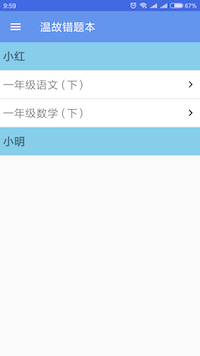
\includegraphics{img/18.png}
	\caption{主界面}
	\label{img18}
\end{figure}
现在在小红的错题本“一年级数学(下)”里面添加错题,点击“一年级数学(下)”条目进入错题本,如图(\ref{img19})
\begin{figure}[H]
	\centering
	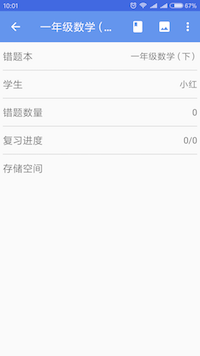
\includegraphics{img/19.png}
	\caption{一年级数学(下)}
	\label{img19}
\end{figure}
此页面显示了错题本名、学生名、错题数量、复习进度(已经复习/错题数量)、存储空间。

右上角是几个操作按钮、分别是复习、相册选取、拍照、重置。

\subsubsection{增加错题}
步骤1:可以选择“相册选取”或“拍照”获得一张错题照片。建议手机横拍。这里需要权限(拍摄照片、存储等),请允许。
\begin{itemize}
	\item 相册选取(建议,效率更高。先集中一起拍照,然后从相册中一张张选择处理)
	\item 拍照(拍一张,处理一张)
\end{itemize}

步骤2:把照片裁剪到合适的大小,如图(\ref{img20})。满意点击右上角\Checkmark ,进入裁剪。不满意,点击左上角\XSolid ,退回错题本。

\begin{figure}[H]
	\centering
	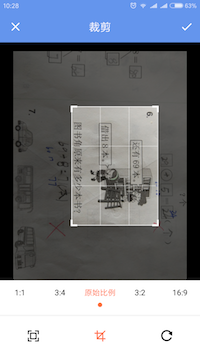
\includegraphics{img/20.png}
	\caption{裁剪}
	\label{img20}
\end{figure}

步骤3:涂改掉多余的答案等,仅保留题干,如图(\ref{img21})。左上角回退菜单会退回到错题本。右上角第一个是撤销一次涂改,第二个是进入步骤4。
\begin{figure}[H]
	\centering
	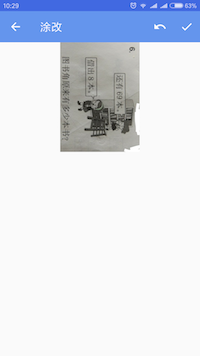
\includegraphics{img/21.png}
	\caption{涂改}
	\label{img21}
\end{figure}

步骤4:如图(\ref{img22}),就是复习是会看到的错题。可选操作,右上角有3个按钮,分别是错解、正解、总结,可以为这道错题添加上错误的解法、正确的解法、自己的归纳总结等(还是通过“拍照→剪切→涂改→保存”这个步骤录入。)。如果不需要额外增加信息,可以直接点击左上角回退到错题本。
\begin{figure}[H]
	\centering
	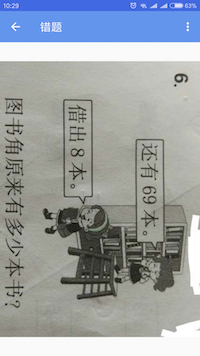
\includegraphics{img/22.png}
	\caption{错题浏览}
	\label{img22}
\end{figure}

现在的错题本看上去是这样,如图(\ref{img23})
\begin{figure}[H]
	\centering
	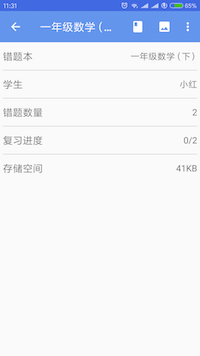
\includegraphics{img/23.png}
	\caption{错题本}
	\label{img23}
\end{figure}

\subsection{复习}
\begin{figure}[H]
	\centering
	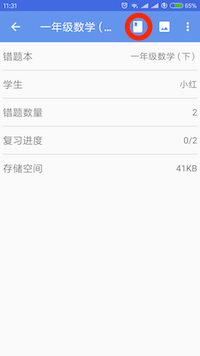
\includegraphics{img/24.png}
	\caption{进入复习}
	\label{img24}
\end{figure}

点击“复习”菜单,如图(\ref{img24}),进入复习页面,如图(\ref{img25})。这里是随机复习模式,低年级学生在家长陪同的情况下使用,因为需要随时批改。不能随时批改的情况下,建议使用“测验模式”。

\begin{figure}[H]
	\centering
	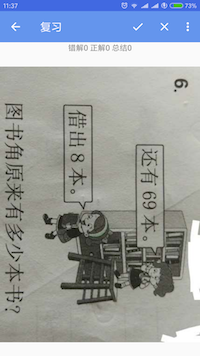
\includegraphics{img/25.png}
	\caption{复习}
	\label{img25}
\end{figure}

随机从未复习的错题中选择一题,根据本次答题情况,分别选择\Checkmark 或 \XSolid 按钮。回答正确的,本轮复习中不会再次出现。

右上角下拉菜单中,有错解、正解、总结按钮,可以这时增加当前错题的错解、正解、总结。移动按钮可以移动当前错题到其他错题本中。删除按钮,可以删除当前错题。

\subsection{测验}
批量复习,批量批改。
\begin{figure}[H]
	\centering
	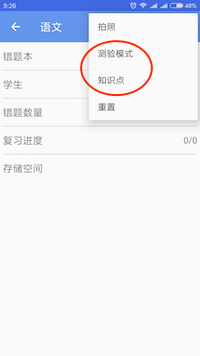
\includegraphics{img/32.png}
	\caption{进入测验}
	\label{img32}
\end{figure}
点击“测验模式”菜单进入测验列表,如图(\ref{img32})

点击右上角“+”,选择本次测验的题目数量,增加新测验,如图(\ref{img33})。
\begin{figure}[H]
	\centering
	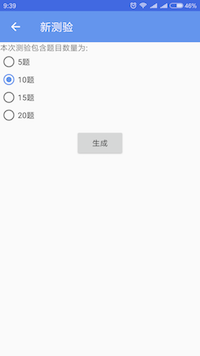
\includegraphics{img/33.png}
	\caption{新测验}
	\label{img33}
\end{figure}

从测验列表(\ref{img34})进入测验复习
\begin{figure}[H]
	\centering
	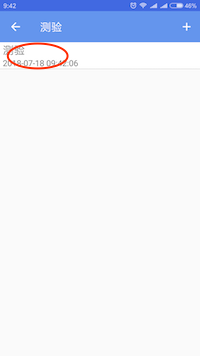
\includegraphics{img/34.png}
	\caption{测验列表}
	\label{img34}
\end{figure}

学生通过右上角上下箭头,切换题目,(\ref{img35})
\begin{figure}[H]
	\centering
	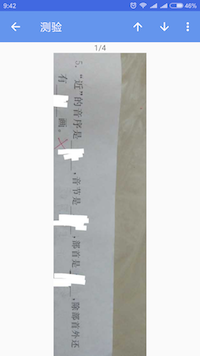
\includegraphics{img/35.png}
	\caption{测验}
	\label{img35}
\end{figure}

家长可以通过右上角菜单“批改模式”,进入批改状态,如图(\ref{img36})
\begin{figure}[H]
	\centering
	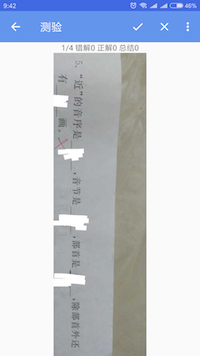
\includegraphics{img/36.png}
	\caption{测验批改}
	\label{img36}
\end{figure}
根据本次答题情况,分别选择\Checkmark 或 \XSolid 按钮。回答正确的,本轮复习中不会再次出现。可以这时增加当前错题的错解、正解、总结。删除是删除当前测验。

\subsection{知识点}
进入知识点列表,如图(\ref{img37})
\begin{figure}[H]
	\centering
	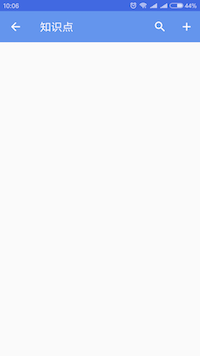
\includegraphics{img/37.png}
	\caption{知识点列表}
	\label{img37}
\end{figure}
点击右上角“+”,进入增加页面,如图(\ref{img38})。放大镜图标,可以按标题搜索。
\begin{figure}[H]
	\centering
	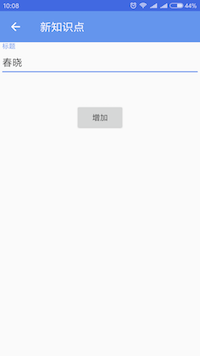
\includegraphics{img/38.png}
	\caption{增加知识点}
	\label{img38}
\end{figure}
在知识点列表中,点击刚刚增加的“春晓”,进入知识点页面,如图(\ref{img39})
\begin{figure}[H]
	\centering
	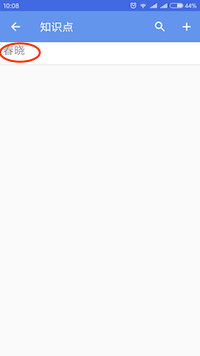
\includegraphics{img/39.png}
	\caption{知识点}
	\label{img39}
\end{figure}
现在可以通过拍照、相册选取,加入多张知识点图片,如图(\ref{img40})
\begin{figure}[H]
	\centering
	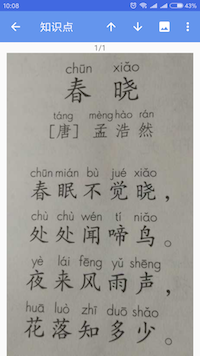
\includegraphics{img/40.png}
	\caption{知识点}
	\label{img40}
\end{figure}
上下箭头,可以在多张图片中切换。删除可以删除一张图片。删除知识点可以删除当前知识点。

\subsection{重置}
\begin{figure}[H]
	\centering
	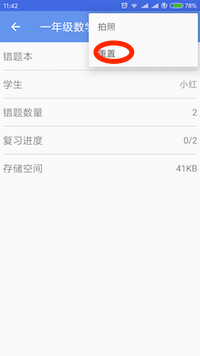
\includegraphics{img/26.png}
	\caption{重置}
	\label{img26}
\end{figure}
错题本中的错题全部复习完成,点击如图(\ref{img26})按钮可以重新重置错题状态为可复习状态。